% !TeX spellcheck = ru_RU
% !TEX root=../main.tex

\begin{lecture}[Электролитическая диссоциация]
\begin{lecSection}[Равновесия в водных системах]
	Как было показано в прошлой лекции, 
	\begin{gather*}
		\sum\limits_{j=1} \nu_j' A_j' - \sum\limits_{j=1} \nu A = 0 \\
		K = \prod\limits_{k} C_k^{\nu_k},  \tab K = \exp\left( -\dfrac{\Delta G^0}{RT} \right) \\
		\Delta G^0 = \sum\limits_{k} \nu_k' \mu_k^{0'}
		- \sum\limits_l \nu_l \mu_l^0 \\
		K \simeq Z \cdot \exp\left( -\dfrac{\Delta G^0}{RT} \right) \\
	\end{gather*}
	Рассмотрим переход $ R \xrightarrow{K} P $
	
	\begin{figure}[H]
	\begin{minipage}[h]{0.26\linewidth}
		\centering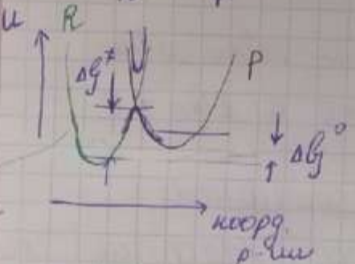
\includegraphics[width=\linewidth]{lecture_04/graph1}
	\end{minipage}
	\hfill
	\begin{minipage}[h]{0.30\linewidth}
		\centering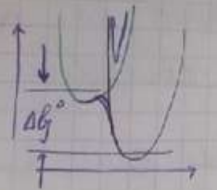
\includegraphics[width=\linewidth]{lecture_04/graph2}
	\end{minipage}
	\hfill
	\begin{minipage}[h]{0.28\linewidth}
		\centering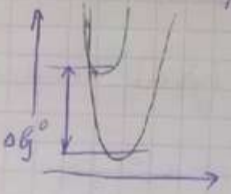
\includegraphics[width=\linewidth]{lecture_04/graph3}
	\end{minipage}
	\caption{Возможные случаи расположения термов}
	\end{figure}

	Рассмотрим две молекулы $ D, A $:
	\begin{equation*}
		D + A \rightarrow D^{+} + A^{-}
	\end{equation*}
	Имеется несколько путей ионизации. Они приведены на рис. \ref{fig:possible_ways_of_ionization}
	\begin{wrapfigure}{l}{0.4\linewidth}
		\centering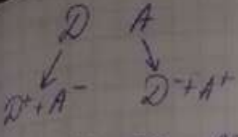
\includegraphics{lecture_04/diag1}
		\caption{Возможные пути ионизации}
		\label{fig:possible_ways_of_ionization}
	\end{wrapfigure}
	Вводится характеристика $ IP $ -- потенциал ионизации и $ AE $ -- сродство к электрону.
	\begin{gather*}
		IP_D - AE_A < IP_A - AE_D \\
		IP_A + AE_A > IP_D + AE_D \\
		\text{ (хотим ли из A сделать донора?) } \\
		D - \pi - A
	\end{gather*}
	Примером этого может служить DASPI (рис. \ref{fig:daspi})
	
	\begin{figure}[h]
		\centering
		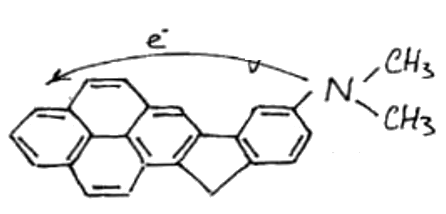
\includegraphics[width=0.7\linewidth]{lecture_04/new_daspi}
		\caption[Молекула DASPI]{Молекула DASPI}
		\label{fig:daspi}
	\end{figure}
	
	\begin{center}\begin{tabular}{cl}
		$ K_A \text{ (константа диссоциации)}$ & $HA \leftrightarrow H^+  + A^- $ \\
		$K_B$ & $MOH \rightleftharpoons M^+ + OH^- $ \\
		\multicolumn{2}{c}{$\text{pH раствора} $} \\
		$pH = - \lg [H^+]$ & $pX = - \lg [X] $ \\
		\multicolumn{2}{c}{$H_2O \rightleftharpoons H^+ + OH^- $} \\
	\end{tabular}\end{center}
	\begin{center}\begin{tabular}{ll}
	$ \overset{\sim}{K} = \dfrac{[H^+][OH^-]}{[H_2O]} $ & $ [H_2O] = \text{const} $ \\
	$ K_w = \overset{\sim}{K} [H_2O] = [H^+][OH^-]; $ & $ K_w = f(T) $ \\
	$ t = 20 - 25 ^\circ C $ & $ -\lg K_w = 14 $ \\
	$ [H^+][OH^-]; $ & $ K_w = [H^+]^2 $
	\end{tabular}\end{center}
	\[ -2 \lg [H^+]  = 14 ~~ \rightarrow ~~ pH = 7 \]
	При $ pH < 7 $ среда является кислотной.
	\begin{gather*}
	H_2 CO_3 \rightleftharpoons H^+ + HCO_3^- \\
	OH^- + H_2 CO_3 \rightarrow HCO_3^- + H_2O
	\end{gather*}
	
	\textbf{Принцип Ле-Шателье}: если на систему, находящуюся в устойчивом равновесии, воздействовать извне, изменяя какое-либо из условий равновесия (температура, давление, концентрация, внешнее электромагнитное поле), то в системе усиливаются процессы, направленные в сторону противодействия изменениям.
	
	\begin{tabular}{ll}
		$ H_3O^+ $ & (Volmer, 1924) \\
		$ H_2 OH^+ OH_2 $ & (Zundel, 1976)
	\end{tabular}

	\begin{figure}[h]
		\centering
		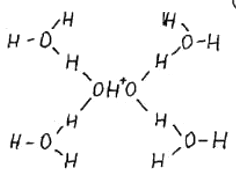
\includegraphics[width=0.4\linewidth]{lecture_04/new_k_molec}
		\caption[Вид гидратированного комплекса]{Вид гидратированного комплекса}
		\label{fig:kmolec}
	\end{figure}

	\begin{definition}
		Сольватация --- взаимодействие растворенных частиц с молекулами растворителя.
	\end{definition}
\end{lecSection}

	\begin{lecSection}[Буферные системы]
		\begin{definition}
			Буфер --- раствор, способный сохранять $ pH $ при добавлении в него кислоты, щелочи или разбавлении раствора.
		\end{definition}
	При этом $ [HA]_0 = a $ -- слабая кислота. Либо $ [MOH]_0 = b $ -- слабое основание.
	
	В случае, когда $ [HA] $ полностью диссоциирована:
	\begin{enumerate}
		\item $ a = [HA] + [A^-] $
		\item $ b + [H^+] = [A^-] + [OH^-] $
	\end{enumerate}

	\begin{equation*}
		K_A = \dfrac{[H^+] [A^-]}{[HA]} = 
		\dfrac{[H^+] [A^-]}{a - [A^-]} ~~ \rightarrow ~~ 
		[A^-] = \dfrac{a K_A}{K_A + [H^+]}
	\end{equation*}
	
	\begin{equation}
	\boxed{
		b = \dfrac{a K_A}{K_A + [H^+]} - [H^+] + \dfrac{ K_w }{ [H^+] }
	}
	\label{eq:b_in_buffer}
	\end{equation}
	\end{lecSection}
	
\end{lecture}
